\documentclass[../main.tex]{subfiles}

\begin{document}
Para poder empezar con el modelado en Protegé se ha considerado como clases todas las características dentro del documento llamado \textbf{medicamentos.xlsx } tal y como se muestra en la siguiente imagen. Medicamentos se considera la clase principal y el resto de clases heredan de ella.\\

\begin{figure}[h]
    \centering
    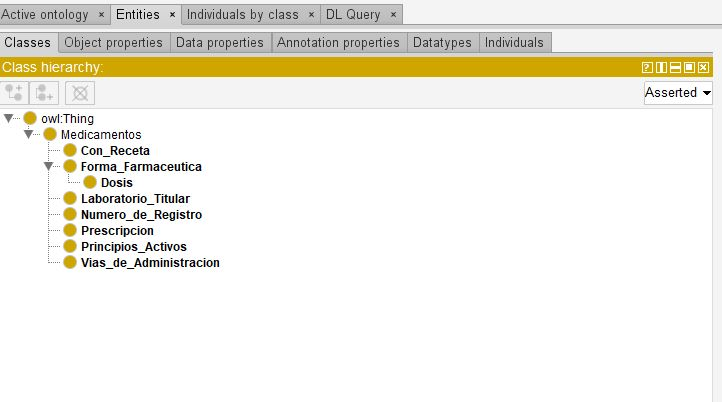
\includegraphics[scale=0.7]{images/protege-Classes.jpeg}
    \caption{Clases}
    \label{fig:mesh1}
\end{figure}


\vspace{2cm}
Se han creado además dos propiedades de tipo objeto que son: como adquirirlo y tipo de laboratorio. La primera tiene como dominio la clase \textbf{Prescripcion} y como rango la clase \textbf{Con-Receta}. La segunda tiene como dominio la clase de \textbf{Laboratorio Titular}.\\

\begin{figure}[h]
    \centering
    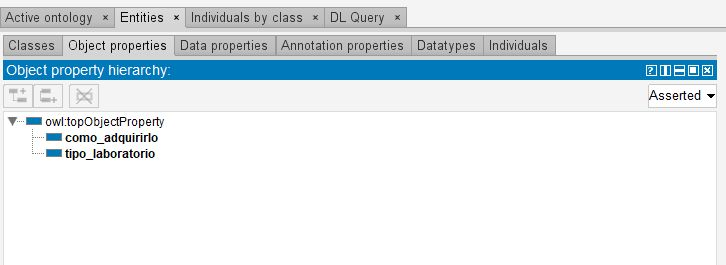
\includegraphics[scale=0.7]{images/protege-ObjectProperties.jpeg}
    \caption{Object Properties}
    \label{fig:mesh1}
\end{figure}

\vspace{1cm}
También, se han creado como propiedades de datos las cinco siguientes: nombre del medicamento que se relaciona con la clase Medicamento directamente, tipos de forma farmaceutica y cantidad de dosis que se relacionan con Dosis, tipos de vías de administración que se relaciona con la clase Vías de Administración y tipos de principios activos que se relaciona con Principios Activos. Todas estas propiedades se han considerado de tipo \textit{string}. \\

\begin{figure}[h]
    \centering
    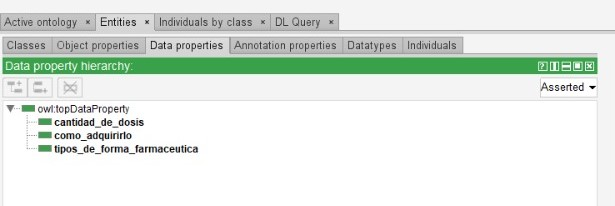
\includegraphics[scale=0.7]{images/protege-DataProperties.jpeg}
    \caption{Data Properties}
    \label{fig:mesh1}
\end{figure}

\vspace{2cm}
Se ha creado un ejemplo de medicamento en el que se han insertado datos para las propiedades de datos y se ha seleccionado de que tipo de clase es dicho individuals. \\

\begin{figure}[h]
    \centering
    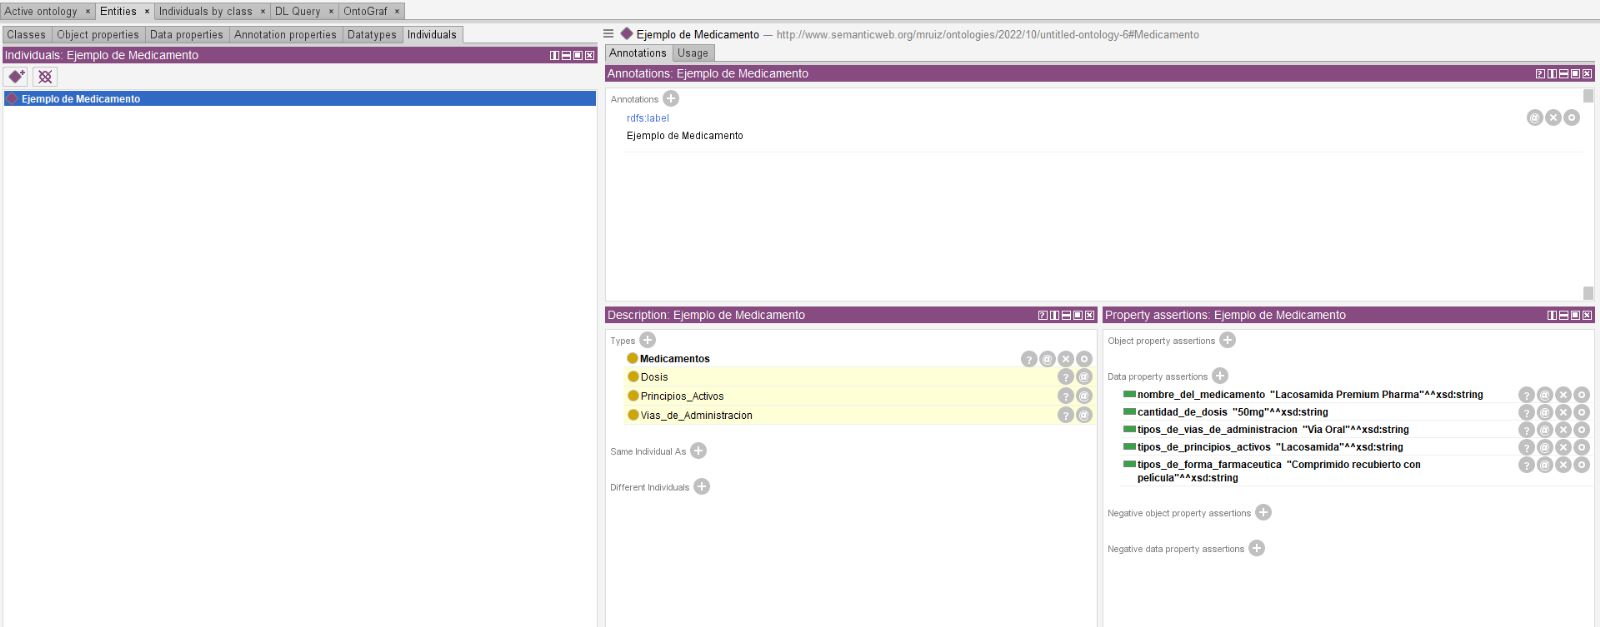
\includegraphics[scale=0.4]{images/protege-Annotations.jpeg}
    \caption{Annotations}
    \label{fig:mesh1}
\end{figure}

\vspace{1cm}
Finalmente, se ha generado un grafo con las clases que componen el modelado y el correspodiente ejemplo que hemos creado: \\

\begin{figure}[h]
    \centering
    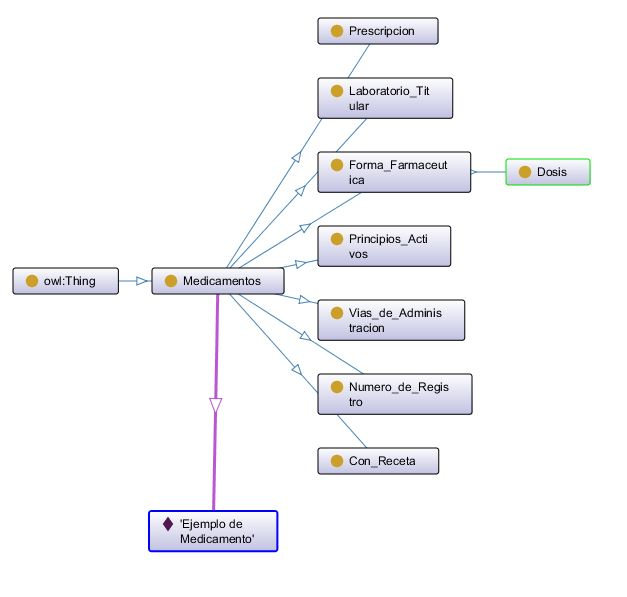
\includegraphics[scale=0.4]{images/protege-Grafo.jpeg}   \caption{Annotations}
    \label{fig:mesh1}
\end{figure}


\end{document}